%%%%%%%%%%%%%%%%%%%%%%%%%%%%%%%%%%%%%%%%%%%%%%%%%%%%%%%%%%%%%%%%%%%%%%%%%%%%%
% Technical report, NeurIPS 2026 formatting.
% Compile:  latexmk -pdf tech_report.tex   (or: pdflatex twice)
% Figures:  uv run python report/make_figures.py   (writes figures/*.pdf)
% Numbers:  uv run python report/compute_stats.py
%%%%%%%%%%%%%%%%%%%%%%%%%%%%%%%%%%%%%%%%%%%%%%%%%%%%%%%%%%%%%%%%%%%%%%%%%%%%%
\documentclass{article}

% Numeric citations, as in the NeurIPS reference style (see the note in the
% conference template); must precede the style file, which loads natbib.
\PassOptionsToPackage{numbers, compress}{natbib}
\usepackage[preprint]{neurips_2026}

\usepackage[utf8]{inputenc}
\usepackage[T1]{fontenc}
\usepackage{hyperref}
\usepackage{url}
\usepackage{booktabs}
\usepackage{amsfonts}
\usepackage{amsmath}
\usepackage{amssymb}
\usepackage{nicefrac}
\usepackage{microtype}
\usepackage{xcolor}
\usepackage{graphicx}
\usepackage{caption}
\captionsetup{font=small}

\newcommand{\eot}{\texttt{<|endoftext|>}}

\title{A Transformer Language Model From Scratch:\ Implementation and Controlled Experiments}

\author{%
  Yi Hou \\
  University of Chinese Academy of Sciences\\
  Beijing, China \\
  \texttt{houyi25@mails.ucas.ac.cn} \\
}

\begin{document}

\maketitle

\begin{abstract}
This report documents a from-scratch implementation of everything needed to train a Transformer language model --- a byte-level BPE tokenizer, the model (RMSNorm, RoPE, SwiGLU, causal attention), AdamW with warmup and cosine decay, and the training loop --- written without the corresponding PyTorch and HuggingFace building blocks, and cross-checked against them where a reference exists. I train a 22.7M-parameter model on TinyStories (4 layers, $d_{\text{model}}{=}512$, 327.7M tokens seen) and report a learning-rate sweep, a batch-size sweep at a fixed token budget, one main run reaching 1.57 validation loss in 1.5 GPU-hours, and four ablations. The ablations reproduce the expected qualitative picture: removing RMSNorm makes training diverge to NaN within 250 steps --- and lowering the learning rate 10$\times$ restores stability but not quality (3.94 vs.\ 2.19 at a matched step) --- removing rotary embeddings costs 0.48 nats, post-norm is slightly worse than pre-norm, and SwiGLU and SiLU land within 0.03 nats once parameter counts are matched (22.70M vs.\ 22.83M). Two findings are less expected. First, extending the learning-rate sweep to 1{,}000$\times$ the optimum never produces a NaN \emph{final} loss, because the cosine tail anneals every run back to a safe regime --- the divergent runs are visible only in the trajectory (one reaches $6\!\times\!10^{3}$ mid-training) and a control with the learning rate held constant never recovers. Second, training the tokenizer on the full 1.92\,GB corpus takes 99.6\,s and peaks at 9.5\,GiB, with ~85\% of the time in the merge-selection scan rather than in pretokenization. I also report tokenizer statistics (4.18 bytes/token, 15-byte longest token) and state plainly which parts of the planned study I did not attempt.
\end{abstract}

\section{Introduction}
\label{sec:intro}

This report documents a from-scratch implementation study of a language-modeling stack: a byte-level BPE tokenizer, a Transformer language model, an AdamW optimizer with a learning-rate schedule, and a training loop, each written without the library component that would normally do the job --- followed by controlled experiments on a small model. The point of the exercise is not to produce a competitive model but to make every design decision in a modern LLM stack something I have had to write down myself.

\paragraph{Scope.} The following are written from scratch, in the sense that no library implementing that specific function is used: the BPE tokenizer (all of it --- pretokenization, training, encoding, decoding), the model (embedding, RMSNorm, rotary position embeddings, causal multi-head attention, SwiGLU feed-forward, residual stream), the loss (cross-entropy computed without materializing a softmax), the optimizer (AdamW, including the decoupled weight decay and the bias-corrected moments), the learning-rate schedule, gradient clipping, checkpointing, the data loader, and the sampling decoder. What I do use is autograd, tensor primitives, \texttt{torch.nn.Parameter}, the generic \texttt{torch.optim.Optimizer} base class, \texttt{regex}, and multiprocessing. In particular, no \texttt{nn.Transformer}, \texttt{nn.MultiheadAttention}, \texttt{nn.RMSNorm}, \texttt{torch.optim.AdamW}, or HuggingFace tokenizer is used in the training path.

\paragraph{What this report is.} Section~\ref{sec:impl} describes the implementation; Section~\ref{sec:setup} fixes the experimental setup; Section~\ref{sec:results} reports the sweeps, the main run, generations, and four ablations; Section~\ref{sec:discussion} discusses what the numbers mean and lists limitations, including the parts of the study I deliberately did not do. Two caveats up front, because they affect how the numbers should be read. First, every run here is a \emph{single} run of a single-GPU job on one NVIDIA A6000 (the sweeps and ablations were spread across six such GPUs, but each individual run is one GPU); no random seed is fixed in the training script, so differences below $\sim$0.06 nats between two runs of the same configuration are not meaningful. Second, the model is small --- 22.7M parameters, trained on a 1.9\,GB synthetic corpus --- so nothing here is a scaling result.

\section{Implementation}
\label{sec:impl}

\subsection{Byte-level BPE tokenizer}

\paragraph{Pretokenization.} Text is split with the GPT-2 split pattern \citep{bpe,gpt2} (contractions, then runs of letters, digits, and other characters, with leading spaces attached) into pretokens, and each pretoken is converted to a byte sequence using the GPT-2 byte-to-unicode mapping, so that every one of the 256 byte values is one printable character. Merges never cross a pretoken boundary, which is what keeps the tokenizer's behaviour on whitespace and punctuation predictable. Special tokens are split out \emph{before} pretokenization (longest-first alternation) and mapped to their own ids.

\paragraph{Training.} Counting all adjacent symbol pairs over the corpus, then rescanning after every merge, is correct but quadratic. The implementation instead builds a pretoken $\rightarrow$ frequency counter once, and then maintains a reverse index from each adjacent pair to the set of pretokens containing it, together with that pair's total count. Each merge updates only the counter entries and reverse-index sets touched by the occurrences of the merged pair, so the cost of a merge scales with the number of affected occurrences rather than with corpus size. The winning pair each round is the one with the largest count, with ties broken by the lexicographically larger pair, matching the reference implementation used in the correctness checks below. Pretokenization of a large file is parallelized over byte ranges aligned to \eot{} boundaries, so the corpus is still treated as one document stream.

Two correctness checks: a reference test suite compares my merges and vocabulary against a reference tokenizer trained on a fixture corpus, and a separate script diffs my output against the reference files token-by-token, requiring exact equality. Both pass: the tokenizer is \emph{bit-exact} with the reference on the fixture, i.e.\ the merge order is identical, not merely equivalent.

\paragraph{Measured statistics.} Trained on TinyStories \citep{tinystories} with a target vocabulary of 10{,}000 and \eot{} as the only special token, the tokenizer produces 10{,}000 entries and 9{,}743 merges. Its longest token is 15 bytes (e.g.\ \texttt{\textvisiblespace{}accomplishment}, \texttt{\textvisiblespace{}disappointment}); 2{,}375 of the 10{,}000 tokens are at least 8 bytes and 131 are at least 12 bytes. This is what one should expect from this corpus: the longest tokens are ordinary long English words that appear often enough in simple stories to be merged, and because merges cannot cross pretoken boundaries no pathological whitespace-spanning token exists. Compression is 4.18 bytes/token over the full training corpus (1.92\,GB $\rightarrow$ 460.4M tokens) and 4.01 bytes/token on 10 sampled validation documents (range 3.76--4.27). Encoding runs at 0.72\,MB/s (172K tokens/s) on the training host --- slightly \emph{slower} than on the laptop used for the earlier measurements, because encoding is single-threaded Python and this host's single-core clock is lower. Extrapolated, tokenizing the 825\,GB Pile \citep{pile} would take roughly 14 days in a single process, which is why the tokenized corpus is cached as a NumPy array. That cache is \texttt{uint16}: the vocabulary is 10{,}000, far below $2^{16}$, so every token id fits, and the training tokens occupy 921\,MB instead of 1.8\,GB in \texttt{int32}.

\paragraph{What training the tokenizer costs.} Training the full 1.92\,GB corpus with a 10{,}000-token vocabulary takes 99.6\,s of wall clock on a 64-core machine (against a reference budget of 30 minutes on a 16\,GB machine) and peaks at 9.5\,GiB of resident memory summed over the process tree. Profiling a 200\,MB subset says where that time goes: the merge loop accounts for about 85\% of it --- 74.9\,s of 85.7\,s, essentially all inside the scan for the highest-count pair (10{,}502 calls, 232M comparison-lambda calls) --- while parallel pretokenization is the remaining 14\%. The same merge loop costs about the same on the full corpus, so the dominant term here is the per-merge argmax scan rather than the corpus-side work, and replacing that scan with a heap or a bucketed count structure is the obvious next step. We did not implement that, which is why the reported wall clock is a measurement rather than a best effort.

\subsection{Model}

The model is a decoder-only Transformer \citep{transformer} in the pre-norm style, with four deliberate modernizations, and it is deliberately small.

\begin{itemize}
  \item \textbf{RMSNorm} \citep{rmsnorm} before each sublayer (and once more before the output projection), computed in \texttt{float32} and applied to the last axis.
  \item \textbf{Rotary position embeddings} \citep{rope} (\texttt{theta}{=}10{,}000) applied to queries and keys, with $\cos/\sin$ tables precomputed as non-persistent buffers and applied to the interleaved $(2k, 2k{+}1)$ coordinate pairs.
  \item \textbf{SwiGLU} \citep{swiglu} as the feed-forward: $\mathrm{SiLU}(xW_1) \odot xW_3$ projected back by $W_2$, with $d_{ff} = 1344$ rather than the classic $4d_{\text{model}}$.
  \item \textbf{Causal attention} with an explicit lower-triangular mask applied as $-\infty$ before a hand-written softmax, which is computed by subtracting the row maximum first.
\end{itemize}

There is no KV cache and no fused attention kernel: each attention head materializes its full $T \times T$ score matrix, and generation re-runs the model on the whole prefix for every new token. That is the right trade for a from-scratch baseline --- the arithmetic is visible and the training path has no hidden kernels --- and it is one of the reasons generation is slow relative to training.

Initialization is truncated normal with $\sigma = \sqrt{2/(d_{in}+d_{out})}$ for linear layers and $\sigma=1$ for embeddings, truncated at $\pm 3\sigma$. The token embedding and the output projection are untied. The resulting model has 22.70M parameters (5.12M embedding, 5.12M output projection, 12.45M in the four blocks), i.e.\ 87\,MiB in \texttt{fp32} parameters alone.

\subsection{Optimizer, schedule, and training loop}

AdamW \citep{adamw} is implemented with the decoupled weight decay applied \emph{before} the moment updates, per-parameter step counters held as tensors, and bias correction applied at every step; the reference tests check it against \texttt{torch.optim.AdamW} to a tolerance of $10^{-4}$ and it passes. The learning-rate schedule is linear warmup followed by cosine decay to a floor of $10^{-5}$, with warmup set to 5--10\% of the run (100 steps in the 1{,}000-step sweeps and the 2{,}000-step ablations, 250 steps in the 5{,}000-step main run). Gradients are clipped by global $\ell_2$ norm at 1.0 before every optimizer step. Batches are drawn as random offsets into a memory-mapped token array, so the 1.9\,GB corpus never has to be held in RAM, and checkpoints save model, optimizer, and iteration so that a killed run can be resumed.

\subsection{Cross-checking against production libraries}
\label{sec:xcheck}

A from-scratch implementation that only passes its own tests is not evidence of anything, so each component is also checked against the library that would normally do the job:

\begin{itemize}
  \item \textbf{Tokenizer}: tiktoken's GPT-2 encoding, compared byte-exactly on TinyStories text (the tiktoken cache is seeded offline and verified by SHA-256); and a second, independently trained tokenizer built with HuggingFace \texttt{tokenizers} \citep{hf} (BPE + ByteLevel) at vocabulary 1{,}000 for a structural comparison.
  \item \textbf{Optimizer}: the reference test suite's comparison against \texttt{torch.optim.AdamW}, plus the reference implementation's own loop using \texttt{torch.optim.AdamW} with \texttt{SequentialLR} over \texttt{LinearLR} and \texttt{CosineAnnealingLR}.
  \item \textbf{Model}: an end-to-end training run on \texttt{transformers.GPT2LMHeadModel} with \texttt{torch.optim.AdamW}, \texttt{F.cross\_entropy}, \texttt{clip\_grad\_norm\_}, and a \texttt{DataLoader} --- deliberately \emph{not} architecture-identical (GPT-2 is post-norm with GELU and learned absolute positions), so the comparison is about the training plumbing rather than a bitwise match.
  \item \textbf{Accounting}: a parameter/FLOP accounting script that computes what the model should cost and what the hardware should deliver, used as a sanity check on the measurements above.
\end{itemize}

The value of this exercise turned out to be diagnostic rather than ceremonial: the byte-exact tiktoken comparison is what caught an early divergence in merge-order tie-breaking, and the \texttt{AdamW} comparison caught the weight-decay/direction ordering.

\section{Experimental setup}
\label{sec:setup}

\paragraph{Data.} The original TinyStories release \citep{tinystories}: 1.92\,GB of training text and 19.4\,MB of validation text, tokenized with the 10{,}000-token BPE vocabulary above into 460.4M and 4.6M tokens. (The TinyStories release documentation points at the V2-GPT4 variant; the runs reported here used the original release --- see Section~\ref{sec:discussion}.) Documents are separated by \eot{}.

\paragraph{Model and training.} Table~\ref{tab:config} lists the configuration. All runs use context length 256, AdamW with $\beta=(0.9, 0.999)$, $\epsilon=10^{-8}$, weight decay 0.01, and gradient-norm clipping at 1.0; the only things varied across experiments are the learning rate, the batch size, and the ablated component. Each run is a single process on one A6000 (48\,GB); runs within a sweep were distributed over six GPUs so that a sweep finishes in the time of its longest member.

\begin{table}[t]
\caption{Model and training configuration for all reported runs. Ablations change one row at a time, as noted in Section~\ref{sec:ablations}.}
\label{tab:config}
\centering
\small
\begin{tabular}{@{}ll@{}}
\toprule
Parameter & Value \\
\midrule
Vocabulary & 10{,}000 \\
Context length & 256 (512 at generation) \\
Layers & 4 \\
$d_{\text{model}}$, heads & 512, 16 ($d_{\text{head}}{=}32$) \\
$d_{ff}$ (SwiGLU) & 1{,}344 \\
Positional encoding & RoPE, $\theta{=}10^4$ \\
Parameters & 22.70M \\
\addlinespace
Optimizer & AdamW, $\beta{=}(0.9,0.999)$, $\epsilon{=}10^{-8}$ \\
Weight decay & 0.01 \\
Gradient clipping & global $\ell_2$ norm, 1.0 \\
Schedule & linear warmup, cosine to $10^{-5}$ \\
Warmup & 100 steps (1k/2k-step runs), 250 (5k) \\
Batch size $\times$ context & 64 or 256 $\times$ 256 tokens \\
Hardware & 1 $\times$ NVIDIA A6000 (48\,GB) per run \\
\bottomrule
\end{tabular}
\end{table}

\paragraph{What is measured.} Validation loss is the mean cross-entropy over 10 batches of 256 sequences drawn at random from the validation token array, which makes it itself a random quantity at the $10^{-3}$ level; I did not compute error bars. Training loss shown in figures is the loss of the single batch used for that step, so it is noisier than the validation curve and should not be read as a trend.

\section{Results}
\label{sec:results}

\subsection{Learning rate}
\label{sec:lr}

Figure~\ref{fig:lr} (left) shows the first sweep: five learning rates at batch size 64 for 1{,}000 steps. Final validation losses are 3.185 ($10^{-4}$), 2.686 ($3\!\times\!10^{-4}$), 2.230 ($10^{-3}$), \textbf{2.185} ($3\!\times\!10^{-3}$), and 3.029 ($10^{-2}$). The curve is not symmetric: on the low side, the loss is still improving when the schedule ends, whereas $10^{-2}$ is \emph{worse} than $10^{-3}$ by a wide margin --- the run is destabilized, though it does not diverge outright. I also tried a second AdamW configuration at $10^{-3}$ --- $\beta_2 = 0.95$ with weight decay 0.1 --- which reached 2.283, worse than the default $\beta_2=0.999$/wd 0.01 (2.230) at this scale.

\begin{figure*}[t]
\centering
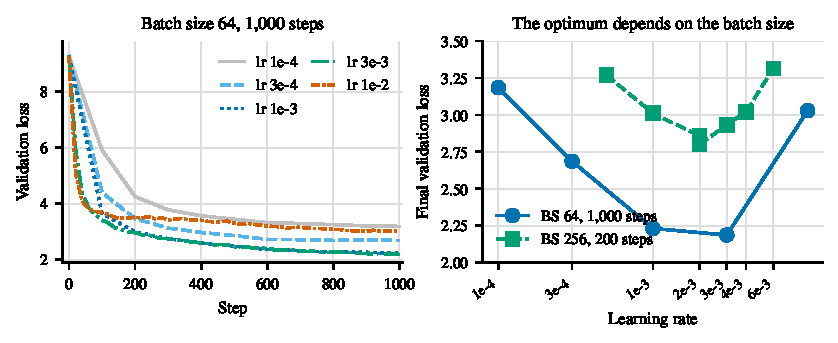
\includegraphics[width=0.93\textwidth]{figures/fig_lr_sweep.pdf}
\caption{Learning-rate sensitivity. \textbf{Left:} validation curves for five learning rates, batch size 64, 1{,}000 steps. \textbf{Right:} final validation loss against learning rate for two sweeps with different batch sizes. The optimum moves from $3\!\times\!10^{-3}$ (batch size 64, 1{,}000 steps) to $2\!\times\!10^{-3}$ (batch size 256, 200 steps), and the penalty for overshooting is steeper than for undershooting. The $2\!\times\!10^{-3}$ point at batch size 256 was run twice; the two runs differ by 0.06 nats (2.798 vs.\ 2.858), which is the run-to-run noise floor in the absence of a fixed seed.}
\label{fig:lr}
\end{figure*}

Because batch size 256 is memory-limited but 8$\times$ the batch, and since larger batches usually want larger learning rates, the sweep was repeated at batch size 256 with a 200-step budget. Here the optimum is $2\!\times\!10^{-3}$ (2.799), with $3\!\times\!10^{-3}$ (2.934) already past the peak and $6\!\times\!10^{-3}$ (3.316) clearly unstable. The shift is visible in Figure~\ref{fig:lr} (right): the 8$\times$ larger batch prefers a $\sim$1.5$\times$ smaller learning rate on this comparison, though the two sweeps differ in both batch size \emph{and} step count, so this is not a clean scaling statement --- it is the practical reason I re-swept at all.

\paragraph{How far the learning rate can go before training breaks.} The sweep above stops at $10^{-2}$, where the run is merely worse (3.029) rather than broken, so I extended it upward at batch size 64: $2\!\times\!10^{-2}$, $3\!\times\!10^{-2}$, $5\!\times\!10^{-2}$, $10^{-1}$, $5\!\times\!10^{-1}$, $1.0$, and $3.0$ --- 1{,}000$\times$ the optimal learning rate --- all with the same 1{,}000-step schedule. The final losses rise monotonically (3.33, 3.96, 4.07, 4.05, 4.78, 5.20, 6.21) and \emph{not one} of these runs ends in NaN. Taken at face value that would say the model tolerates a thousandfold learning rate; the trajectories say otherwise (Figure~\ref{fig:stability}).

The $2\!\times\!10^{-2}$ run is worse but monotone; from $3\!\times\!10^{-2}$ upward the loss rises after warmup before coming back down; and from $5\!\times\!10^{-1}$ the run explodes --- the $1.0$ run peaks near $4\!\times\!10^{2}$ at step 300, the $3.0$ run near $6\!\times\!10^{3}$, and both then descend by orders of magnitude as the cosine tail anneals the learning rate back to $10^{-5}$ over the rest of the run. The divergence is real; the final metric hides it, because the schedule guarantees that every run ends with a tiny learning rate. As a control I reran $0.5$ with the schedule flattened (\texttt{min\_lr}${=}$\texttt{lr}: warmup, then constant), and that run never recovers --- after step 300 it swings between single digits and $4.7\!\times\!10^{2}$ and ends at 88, two orders of magnitude above anything the annealing schedules produce. The divergence threshold for this recipe is therefore around $5\!\times\!10^{-1}$, roughly 170$\times$ the optimal learning rate, and in this setup divergence has to be read off the trajectory rather than the final loss. Note that the threshold is a property of the whole recipe, not of the learning rate alone: removing RMSNorm and changing nothing else breaks training at the \emph{optimal} learning rate of $3\!\times\!10^{-3}$ (Section~\ref{sec:ablations}).

\begin{figure}[t]
\centering
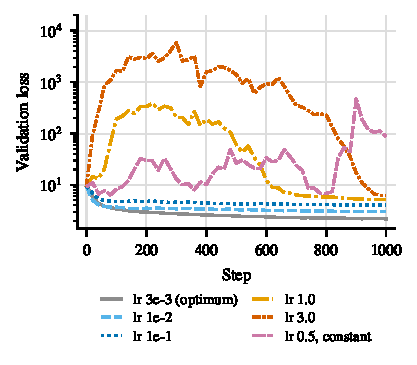
\includegraphics[width=\linewidth]{figures/fig_lr_stability.pdf}
\caption{The same 1{,}000-step schedule at increasing learning rates (batch size 64), on a log scale. Above roughly $5\!\times\!10^{-1}$ the run explodes by two to three orders of magnitude and then recovers as the cosine tail anneals the learning rate back down --- the final losses reported in the text understate how badly these runs behaved in the middle. The purple curve is the control: identical except that the learning rate is held constant, and it never recovers.}
\label{fig:stability}
\end{figure}

\subsection{Batch size at a fixed token budget}

Comparing batch sizes at a fixed \emph{step} count rewards large batches mechanically, so each batch size was run for the same number of tokens (8.4M; 4.2M for batch size 1) at a fixed learning rate of $10^{-3}$. Figure~\ref{fig:bs} shows the result: final validation losses of 2.903 (batch 1, half budget), \textbf{2.414} (32), 2.591 (64), 2.950 (128), 3.396 (256). At a fixed learning rate, larger batches are strictly worse at equal token budget, and the ordering is monotone above batch 32 --- which is the expected signature of a learning rate that is too small for the larger batch, not of large batches being intrinsically worse. Batch size 512 exceeded 48\,GB at context 256 and was not run.

\begin{figure}[t]
\centering
\begin{minipage}[t]{0.48\linewidth}
  \centering
  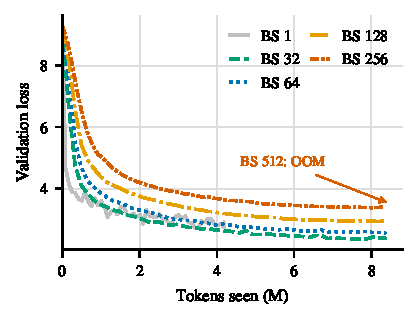
\includegraphics[width=\linewidth]{figures/fig_batch_size.pdf}
  \caption{Batch size at a fixed token budget (8.4M tokens; 4.2M for batch size 1), learning rate $10^{-3}$. Larger batches are worse at equal tokens under a fixed learning rate; batch size 512 ran out of memory.}
  \label{fig:bs}
\end{minipage}\hfill
\begin{minipage}[t]{0.48\linewidth}
  \centering
  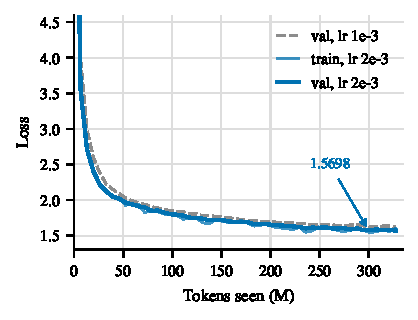
\includegraphics[width=\linewidth]{figures/fig_main_run.pdf}
  \caption{The main run: batch size 256, learning rate $2\!\times\!10^{-3}$, 5{,}000 steps (327.7M tokens, 1.5\,h). Training loss is the per-step batch loss; the dashed curve is the validation loss of the same schedule at $10^{-3}$.}
  \label{fig:main}
\end{minipage}
\end{figure}

\subsection{Main run}

The main run is batch size 256 with the re-swept learning rate $2\!\times\!10^{-3}$ for 5{,}000 steps, i.e.\ 327.7M tokens in about 1.5 hours ($\sim$60K tokens/s). It reaches a final validation loss of \textbf{1.5698} (train 1.5978), against 1.6277 (train 1.6274) for the identical schedule at $10^{-3}$ (Figure~\ref{fig:main}). Re-sweeping the learning rate after changing the batch size was worth about 0.06 nats here --- the same order as the run-to-run noise, which is exactly why I report both numbers rather than the difference.

For calibration: the reference target for this track is 1.45 validation loss on TinyStories. My run does not reach it. The gap is explained by budget rather than by a suspected bug: 1.5 GPU-hours, 5{,}000 steps, and a schedule that ends while the loss is still descending. I kept the setup rather than chasing the target, because the value of the sweeps above is in the comparisons, not in the absolute number.

\subsection{Ablations}
\label{sec:ablations}

Four ablations, each a one-line change to the model, were run with batch size 64 and learning rate $3\!\times\!10^{-3}$ (the batch-size-64 optimum) for 2{,}000 steps, and compared at step 1{,}000 against the unmodified baseline from Section~\ref{sec:lr}. Figure~\ref{fig:abl} shows the curves and the matched-step comparison; Table~\ref{tab:abl} gives the numbers.

\begin{figure*}[t]
\centering
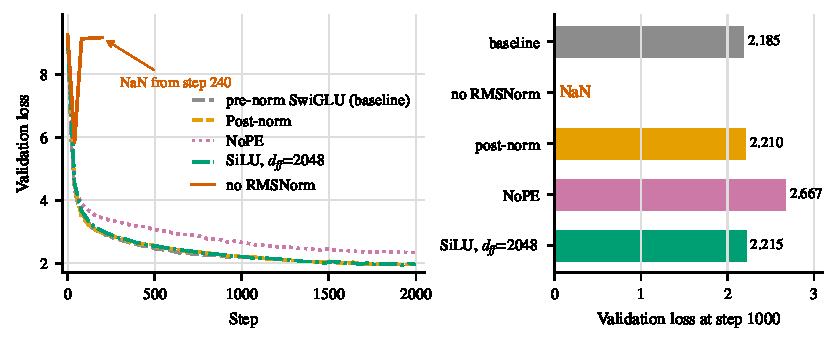
\includegraphics[width=0.93\textwidth]{figures/fig_ablations.pdf}
\caption{Ablations (batch size 64, learning rate $3\!\times\!10^{-3}$). \textbf{Left:} validation curves to step 2{,}000; the dashed grey line is the unmodified model. Removing RMSNorm produces a loss near 9.2 by step 80 and NaN by step 240. \textbf{Right:} validation loss at the matched step 1{,}000, the comparison the runs are designed for.}
\label{fig:abl}
\end{figure*}

\begin{table}[t]
\caption{Ablations at the matched step 1{,}000, batch size 64, learning rate $3\!\times\!10^{-3}$. $\Delta$ is against the baseline. Only the last two columns differ in the number of feed-forward parameters ($d_{ff}$ adjusted so the SiLU variant has the same parameter count as the SwiGLU baseline).}
\label{tab:abl}
\centering
\small
\begin{tabular}{@{}lccc@{}}
\toprule
Variant & Val loss & $\Delta$ & Parameters \\
\midrule
Baseline (pre-norm, SwiGLU) & 2.185 & --- & 22.70M \\
No RMSNorm & \multicolumn{2}{c}{NaN (from step 240)} & 22.70M \\
Post-norm & 2.210 & $+0.025$ & 22.70M \\
NoPE (no rotary) & 2.667 & $+0.482$ & 22.70M \\
SiLU, $d_{ff}{=}2048$ (no gating) & 2.215 & $+0.030$ & 22.83M \\
\bottomrule
\end{tabular}
\end{table}

\begin{itemize}
  \item \textbf{Removing RMSNorm destroys training.} At the previously optimal learning rate the loss is already near 9.2 by step 80 and NaN by step 240. This is the strongest effect of the four and the one that reads as a genuine necessity rather than a preference: without normalization, nothing in this architecture controls activation scale. The natural follow-up question is whether a lower learning rate would rescue it, so I ran two more 2{,}000-step runs: at $10^{-3}$ the loss descends to 5.7 early on and then climbs back toward 9.1 --- the model collapses to something close to uniform predictions --- while at $3\!\times\!10^{-4}$ it trains stably and monotonically to 3.66. So the answer is a qualified yes: a 10$\times$ smaller learning rate buys stability, but the result is 1.7 nats worse than the same model \emph{with} RMSNorm at the matched step 1{,}000 (3.94 vs.\ 2.19). Normalization here is not a stability trick that a smaller step size can substitute for; it is where most of the quality comes from (Figure~\ref{fig:normfollow}).
  \item \textbf{Position information matters a lot.} Dropping RoPE --- leaving the model with no positional signal at all beyond causality --- costs 0.48 nats at the matched step and remains clearly worse at step 2{,}000 (2.351 vs.\ 1.965 for post-norm, which shares its optimizer settings). This is the largest non-diverging effect in the table.
  \item \textbf{Pre-norm beats post-norm slightly}, by 0.025 nats. The gap is small enough to sit near the noise floor, and I would not defend the direction on this evidence alone; it is consistent with the literature but this experiment cannot establish it.
  \item \textbf{SwiGLU and SiLU are indistinguishable at matched parameters.} Replacing the gated feed-forward with a two-matrix SiLU network at $d_{ff}{=}2048$ --- chosen so that the parameter count matches to 0.6\% (22.83M vs.\ 22.70M) --- costs 0.030 nats, again within noise of the pre-norm gap. The honest conclusion is that at 22M parameters on a synthetic corpus, this ablation cannot separate the two; the case for gating is made at larger scale, not here.
\end{itemize}

\begin{figure}[t]
\centering
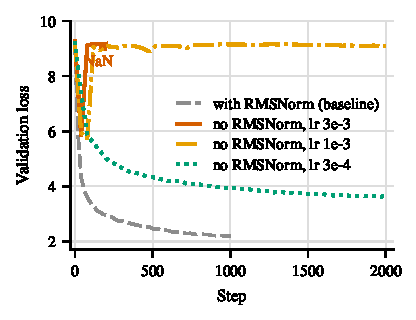
\includegraphics[width=\linewidth]{figures/fig_norm_followup.pdf}
\caption{Removing RMSNorm at three learning rates (batch size 64, 2{,}000 steps). At the optimal $3\!\times\!10^{-3}$ the run diverges to NaN; at $10^{-3}$ it descends and then collapses back toward the uniform-prediction loss $\ln 10^4 \approx 9.2$; at $3\!\times\!10^{-4}$ it trains stably but ends far behind the same model with RMSNorm. A smaller step size buys stability, not parity.}
\label{fig:normfollow}
\end{figure}

\subsection{Generation}

Samples were drawn from the main checkpoint with temperature 0.8 and nucleus sampling at top-$p$ 0.9, for 256 new tokens, using context length 512 --- twice the 256 the model was trained with, a deliberate extrapolation test for RoPE. The prompt \texttt{Once upon a time,} produced:

\begin{quote}
\small
Once upon a time, there was a little boy named Timmy. Timmy loved to play with his toy cars. He had a red car, a blue car, and a yellow car. One day, Timmy was playing with his car when he accidentally broke it. He felt sad and didn't know what to do. Timmy's mom came into his room and saw that he was upset. She asked him what was wrong and Timmy told her about his broken car. His mom told him that they could fix it and they could go to the store to get a new one. \eot{}
\end{quote}

The output is fluent, keeps a consistent cast and tense across eight sentences, and terminates on the end-of-text token where a story would plausibly end. The failure mode that appears over longer generations is semantic rather than grammatical: a story drifts (a toy car becomes a purchase decision becomes a moral about modesty), and repetition of a sentence pattern is common, e.g.\ \emph{``I love you too. Let's go play something else.''} in the \texttt{He looked at} sample. Two factors dominate quality here, and both are structural. First, the model is 4 layers with a 10{,}000-token vocabulary trained on simple stories --- the training data itself is generated text with a narrow register. Second, decoding is temperature-0.8 nucleus sampling with no repetition penalty and no KV cache, and it always emits the full 256 tokens because the generation script passes no end-of-text id to stop on; longer windows accumulate drift that a stopping rule would have hidden. RoPE extrapolation to 512 causes no visible degradation, which is consistent with the design intent of rotary embeddings, though I did not measure validation loss at 512 to confirm it.

\section{Discussion and limitations}
\label{sec:discussion}

\paragraph{What the experiments say.} Three of the four ablations land in the expected direction and the fourth is a null result I would report as such: normalization is load-bearing, positional information is worth a substantial fraction of a nat, pre-norm has at best a small edge, and gating's advantage does not appear at 22M parameters. The most immediately practical result is the batch-size sweep: at a fixed learning rate, batches beyond 32 were worse at equal token budget, and re-sweeping the learning rate recovered 0.06 nats --- batch size and learning rate are not independent knobs.

\paragraph{Two things that surprised me.} First, the learning-rate sweep has no divergent \emph{end state} even at $10^{3}\times$ the optimum, because the schedule's tail rescues every run; the instability is only visible in the trajectory, and a constant-learning-rate control is needed to see a run that stays broken (Section~\ref{sec:lr}). That is a caution about reporting final losses as evidence of stability, including in this report's own earlier sweeps. Second, the tokenizer's cost is not where I assumed: with parallel pretokenization in place, ~85\% of training time is the linear scan for the best pair to merge, and that cost barely moved between a 200\,MB subset and the full 1.92\,GB corpus, because it is set by the number of distinct pairs rather than by how much text they came from. Profiling before optimizing would have saved me from guessing.

\paragraph{Limitations.} Beyond the scale caveats in Section~\ref{sec:intro}: (i) no random seed is fixed, so single runs cannot support small differences, and every $\Delta$ below $\sim$0.06 nats in Table~\ref{tab:abl} is an observation, not a measurement --- this also means the two runs of $2\!\times\!10^{-3}$ at batch size 256 differ by 0.06 nats for no reason other than the seed; (ii) validation loss is computed on 10 random batches, which adds its own sampling noise; (iii) the tokenizer timings come from one run on one host, and the resident-memory figure is the peak of a sampled process-tree sum rather than an instrumented high-water mark.

\paragraph{Not attempted, and deviations.} So that the record is unambiguous: I did not train the tokenizer on OpenWebText and did not run the OpenWebText pretraining track, so the report covers the TinyStories track only. Two deviations are worth stating. The runs here use the \emph{original} TinyStories release (1.92\,GB), not the V2-GPT4 variant the release documentation points at; the tokenizer, the corpus statistics and every model reported above follow from that choice. And the model is a 4-layer, 22.7M-parameter configuration sized to a single A6000, so the absolute losses are not comparable to results obtained with a larger training budget. The remaining planned experiments of the TinyStories track --- BPE training time, memory and profiling, the increasing-learning-rate sweep, and the no-normalization stability question --- are all reported above.

\section{Reproducibility}

The code and this report live in a public repository. Layout: \texttt{lm\_basics/} holds the tokenizer, model, optimizer, loss, data loader, checkpointing, and the training entry point (\texttt{python -m lm\_basics.train}, with \texttt{--transformer\_variant 4a..4d} selecting an ablation); \texttt{tests/} holds the reference test suite and the grading adapters; \texttt{reference\_impl/} holds the library-based cross-checks of Section~\ref{sec:xcheck}; and \texttt{report/} holds this report, the scripts that regenerate its figures (\texttt{make\_figures.py}), its tokenizer statistics (\texttt{compute\_stats.py}), and the tokenizer measurements of Section~\ref{sec:impl} (\texttt{report\_gaps\_bpe.py}). The raw per-step records of every run reported here are kept in \texttt{analysis\_data/} next to the code but are deliberately not committed --- they are bulky and fully regenerable. Because the figures and every number quoted above are produced by the scripts from those records rather than transcribed, the tables cannot drift from the data they summarize: \texttt{make\_figures.py} reprints the exact values cited in the text, so a mismatch between the two would be visible on every rebuild. All training runs use batch size 64 or 256 at context length 256 on one A6000, with the schedule of Section~\ref{sec:impl}; the follow-up runs differ only in the learning rate (and, for the constant-learning-rate control, in \texttt{min\_lr}).

\begin{quote}
\small \emph{Acknowledgement of scope.} This report is an implementation and replication study: the component specifications (the tokenizer's vocabulary and special-token setup, the model architecture, and the experimental protocol of Sections~\ref{sec:lr}--\ref{sec:ablations}) follow established published designs and the reference targets quoted in the text. The implementations, the training pipeline, the measurement protocol, and all results in this report are my own; a reference test suite and a reference tokenizer were used as correctness oracles throughout.
\end{quote}

\begin{thebibliography}{9}

\bibitem{adamw}
Ilya Loshchilov and Frank Hutter.
\newblock Decoupled weight decay regularization.
\newblock \emph{ICLR}, 2019.

\bibitem{bpe}
Rico Sennrich, Barry Haddow, and Alexandra Birch.
\newblock Neural machine translation of rare words with subword units.
\newblock \emph{ACL}, 2016.

\bibitem{gpt2}
Alec Radford, Jeffrey Wu, Rewon Child, David Luan, Dario Amodei, and Ilya Sutskever.
\newblock Language models are unsupervised multitask learners.
\newblock \emph{OpenAI technical report}, 2019.

\bibitem{hf}
Thomas Wolf, Lysandre Debut, Victor Sanh, Julien Chaumond, Clement Delangue, Anthony Moi, Pierric Cistac, Tim Rault, Remi Louf, Morgan Funtowicz, Joe Davison, Sam Shleifer, Patrick von Platen, Clara Ma, Yacine Jernite, Julien Plu, Canwen Xu, Teven Le Scao, Sylvain Gugger, Mariama Drame, Quentin Lhoest, and Alexander Rush.
\newblock Transformers: State-of-the-art natural language processing.
\newblock \emph{EMNLP: System Demonstrations}, 2020.

\bibitem{pile}
Leo Gao, Stella Biderman, Sid Black, Laurence Golding, Travis Hoppe, Charles Foster, Jason Phang, Horace He, Anish Thite, Noa Nabeshima, Shawn Presser, and Connor Leahy.
\newblock The Pile: An 800GB dataset of diverse text for language modeling.
\newblock \emph{arXiv:2101.00027}, 2020.

\bibitem{rmsnorm}
Biao Zhang and Rico Sennrich.
\newblock Root mean square layer normalization.
\newblock \emph{NeurIPS}, 2019.

\bibitem{rope}
Jianlin Su, Murtadha Ahmed, Yu Lu, Shengfeng Pan, Wen Bo, and Yunfeng Liu.
\newblock RoFormer: Enhanced transformer with rotary position embedding.
\newblock \emph{Neurocomputing}, 2024.

\bibitem{swiglu}
Noam Shazeer.
\newblock GLU variants improve transformer.
\newblock \emph{arXiv:2002.05202}, 2020.

\bibitem{tinystories}
Ronen Eldan and Yuanzhi Li.
\newblock TinyStories: How small can language models be and still speak coherent English?
\newblock \emph{arXiv:2305.07759}, 2023.

\bibitem{transformer}
Ashish Vaswani, Noam Shazeer, Niki Parmar, Jakob Uszkoreit, Llion Jones, Aidan N. Gomez, Lukasz Kaiser, and Illia Polosukhin.
\newblock Attention is all you need.
\newblock \emph{NeurIPS}, 2017.

\end{thebibliography}

\end{document}
